\documentclass[]{article}

\usepackage{indentfirst}
\usepackage{titling}
\usepackage{graphicx}
\usepackage{float}
\setlength{\droptitle}{-12em} 

\begin{document}
\title{M.A.S.S \\ Development and Research}
\author{Ben Gotthold}
\date{University of Delaware \\ Spring 2015}
\maketitle

\section{Introduction}

This semester I worked to build and improve an existing implementation of a multi-agent system simulator. I added functionality, validated results, and created agents and simulations to interact with the system. By the end of the semester I was able to run meaningful scenarios with intelligent agents that formed and implemented distinctive plans. I then analyzed the different agent types and evaluated their performance on metrics such as time spent and utility earned. This project presented me with a unique opportunity to understand and implement successful plan formation and agent cooperation within multi-agent systems. 

\section{About the Project}

As technology advances, software is fast becoming the most economical way to test complex solutions to real world problems. Software testing allows a user to run unlimited iterations with complete control over environmental variables. This Multi-Agent System Simulator (M.A.S.S.) was built to provide researchers with the ability to test software agents, allowing them to design more accurate solutions to real world problems faster than ever before.

Although other software simulators exist, the M.A.S.S was developed to be simple, flexible, and completely customizable. With the source code readily available, additional functionality is easy to implement, insuring the system can do what is needed without becoming crowded with unwanted features.

Currently, the M.A.S.S exists as Java executable that uses a ctaems simulation file to produce an environment in which user defined software agents can connect and interact to solve problems. Upon completion, the M.A.S.S. will output the results of the simulation, as well as produce a log detailing the events that occurred within the simulation. While running, the M.A.S.S. allows inter-agent communication and records the number of messages sent by each agent. It is important to note that the M.A.S.S. does not restrict the design of the agents themselves but requires them to adhere to a connection interface so that communication is possible.

\section{Summary of Work}

This section contain a description of the work that was done to improve the existing M.A.S.S as well as the process involved in creating and running different agent-simulation pairs. 

\subsection{Improving the Simulator}
Throughout the course of the semester, I worked to improve existing features and implement new functionality within the M.A.S.S.

\begin{itemize}
\item {\textbf{Time Limit:} Within the optional config.ini a user can now specify the maximum time the simulation will run. By default, this value is 500 time units. This provides protection against a simulation in which the end state is never reached. When the time limit occurs the simulation will terminate, with a time limit warning, providing the user with the utility and duration of the simulation up to that point. }

\item{\textbf{Quality and Duration Distribution:} In the previous version of the M.A.S.S, the system provided each agent with a computed probability of the duration and utility of a given method. It was later found that our experts would be better suited with the agents being provided with the raw distribution only. With this information I collected the raw distributions provided within the ctaems file and passed it to the agents alongside the simulation data. Agents are now free to calculate the expected probability of events themselves. }

\item{\textbf{Aborting a Method:} As agents were formulating and revising plans it became advantageous to allow them to discontinue a method they were running in favor of a more strategic task. To incorporate this I added the ability to abort running methods. When an agent wishes to stop running a method it simply sends an abortMethodMessage to the simulator and the method is terminated. The aborted method can be restarted at any time; however all previous progress made towards completing the method will be lost. }

\item{\textbf{Validation} Throughout the process of adding features and creating agents I was able to provide some validation to the simulator itself. Through my work, I was able to uncover and resolve several bugs, one of which was the way the simulator handled the quality accumulation function OR. By the end of my tests I was able to insure the simulator was working as expected. }

\end{itemize}

\subsection{Building Agents and Scenarios}
Throughout the course of the semester I worked to create unique agent implementations and a diverse set of simulation scenarios to test agents and validate the M.A.S.S.

\begin{itemize}

\item{\textbf{Sprint 1:} I began constructing agents with a python template created by another member of the multi-agent systems lab. This sketch provided the basic framework to send and receive messages with an instance of the simulator running on any machine. To test this design, I first created a random agent. This agent parsed in a description of the simulation and chose an available method at random to complete. I later adapted this agent to create a greedy agent, which completed methods in the order of expected utility. Although it generally preforms better then the random agent, this greedy agent uses no domain knowledge other then the methods that are available to be completed.

\ \ \ \ \ \ \ \  To test these agents, I created a scenario called Test1.ctaems in which a greedy agent could excel. The simulation consisted of three tasks each, with the same three methods related by an OR accumulation function. Since the duration of all 9 methods were the same, a greedy agent should be optimal in this environment. Figure \ref{fig:Tree1} shows a graphical representation of the task tree created by Test1.ctaems.

\begin{itemize}
\item{randomAgent.py}
\item{greedyAgent.py}
\item{Test1.ctaems}
\end{itemize}

\begin{figure}[H]
\caption{A representation of the task tree structure from Test1.ctaems}
\centering
\label{fig:Tree1}
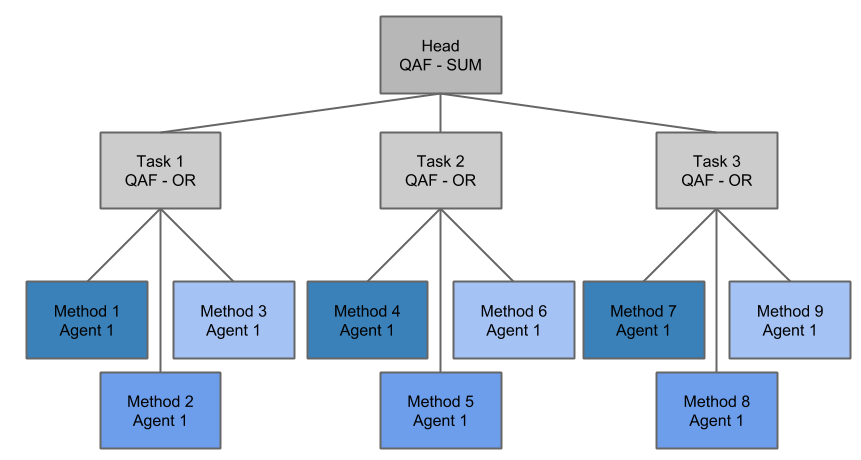
\includegraphics[width=14cm]{images/Tree1.png}
\end{figure}
}

\item{\textbf{Sprint 2:} In this sprint I began constructing an agent that was capable of cooperation. Like before, this agent parsed in the simulation description and began completing methods that would yield the greatest expected utility. This time however, the agent told its peers when it began completing a method, and when that method was complete. In this way, the agent could avoid doing repetitive work. If two methods were predicted to yield the same utility and were related by an OR, only the agent with the smaller load would complete the task. On the other hand, if one agent were expected to yield more from completing a related task, it would ask its neighbor to change focus and work in order to complete a different task. This insured that all OR related methods were done only once by the least busy agent that expected the most utility.

\ \ \ \ \ \ \ \  In Test2.cteams I tested this scenario by creating a task that could be done by any agent for an equal amount of utility. For one agent, this was the only task that it was assigned. By insuring that the agent with the smallest load was the one to complete the task, the total duration of the simulation was decreased. For example, consider a company that received an order for two widgets called A and B. Widget A could be produced by any employee with identical quality and widget B could only be produced by employee X. To minimize the time spent fulfilling the order, it would make sense that an employee other then X produced widget A since X must be the one to produce widget B. Figure \ref{fig:Tree2} shows this example in more detail by depicting the task tree created by Test2.ctaems.

\begin{itemize}
\item{smartAgent1.py}
\item{Test2.ctaems}
\end{itemize}

\begin{figure}[H]
\caption{A representation of the task tree structure from Test2.ctaems}
\centering
\label{fig:Tree2}
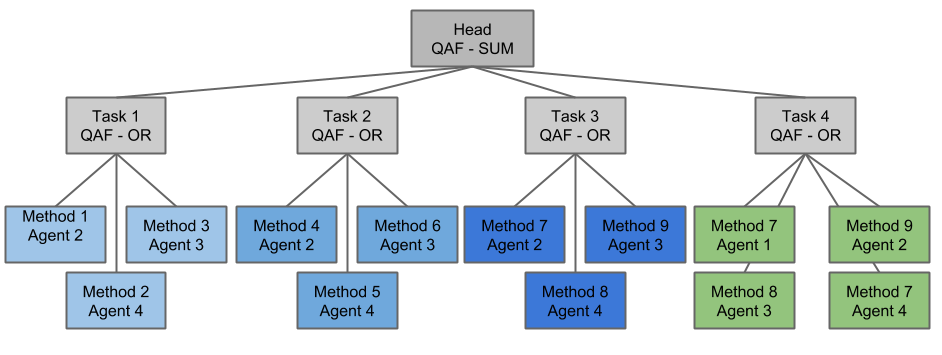
\includegraphics[width=14cm]{images/Tree2.png}
\end{figure}
}
\item{\textbf{Sprint 3:} In this sprint I drastically changed the way agents process the simulation information. Instead of statically parsing the simulation and extracting the methods, agents build a tree to represent the domain as described to them. When agents pass information to one another about the methods they have started and completed they are actually passing parts of the tree. Each agent therefore adds additional pieces to their personal tree to have a better understanding of the simulation as it progresses. This change allows agents to understand how other tasks relate to their own and facilitates decisions that help maximize the total utility.

\ \ \ \ \ \ \ \  In Test3.cteams I tested this scenario by creating a task structure in which all agents could do all tasks however, for every task, one agent was able to do it best. For example, every elementary school teacher specializes in one subject. Each teacher is capable of teaching math, however the most learning occurs when the math teacher is the one to teach the math lesson. This differs from a greedy approach because an agents greedy choice is not the optimal choice in this simulation. Figure \ref{fig:Tree3} shows this example in more detail by depicting the task tree created by Test3.ctaems.

\begin{itemize}
\item{smartAgent2.py}
\item{Test3.ctaems}
\end{itemize}

\begin{figure}[H]
\caption{A representation of the task tree structure from Test3.ctaems. In this tree, Agent\_1's greedy choice is Method 1 however the best choice in that branch is Method 2. Similarly, Agent\_2's greedy choice is Method 6 however the best choice in that branch is Method 7. In this way a greedy agent would not be optimal. }
\centering
\label{fig:Tree3}
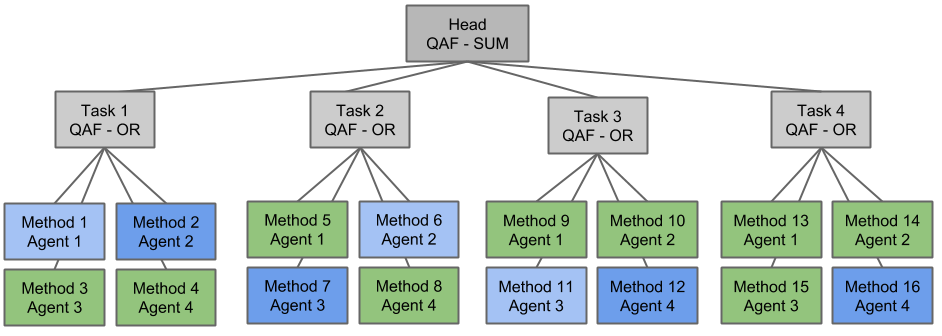
\includegraphics[width=14cm]{images/Tree3.png}
\end{figure}

}

\item{\textbf{Sprint 4:}In the final sprint I created an agent that was capable of planning its path to complete the simulation. Building off my previous work, agents now pass messages to each before the simulation starts. Agents compute what they believe to be the path that maximizes utility and send this plan to their peers. When an agent receives someone else?s plan, they recompute and redistribute their new plan. Eventually the team of agents settles on a plan that is collectively believed to achieve the maximum utility. This allows agents to negotiate relationships and achieve utility that would have previously been stranded.

\ \ \ \ \ \ \ \  In Test4.ctaems I tested this by creating a scenario in which an agent sees a task T that will yield him considerable utility. When he shares his plan to complete task T it is discovered by another agent that T disables task U, a task that will actually yield more quality then task T. In this way, agents preemptively change their plan to maximize total utility. An example of this would be a police officer encountering a criminal. The police officer could arrest the criminal, resulting in one less criminal on the streets. However, if the policeman shares his plan to make the arrest, it may be determined that another agency is actually following the criminal so they can arrest his entire criminal gang. Figure \ref{fig:Tree3} shows this example in more detail by depicting the task tree created by Test4.ctaems.



\begin{itemize}
\item{smartAgent3.py}
\item{Test4.ctames}
\end{itemize}

\begin{figure}[H]
\caption{A representation of the task tree structure from Test4.ctaems. In this tree, Agent\_1's greedy choice is Method 1 however, Method 1 disables Method 6. Similarly, Agent\_2's greedy choice is Method 2, which if completed, will disable Method 12}
\centering
\label{fig:Tree4}
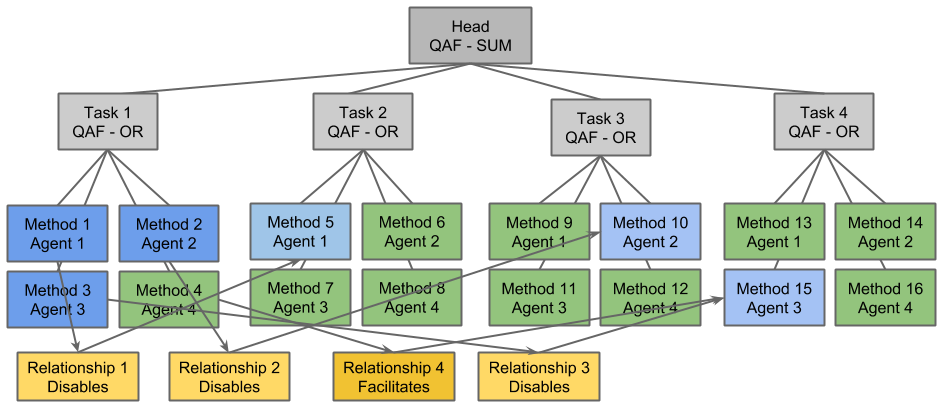
\includegraphics[width=14cm]{images/Tree4.png}
\end{figure}
}

\end{itemize}

\section{Experiment Results}

\begin{itemize}
\item{\textbf{Hypothesis }}

After constructing a variety of agents and environments, I was curious to see how agents would compare across the different simulations I had constructed. The greedy agent was by far the simplest design and faired well in tests conducive to its greedy nature. This led me to wonder if the more complex planning agents were able to outperform the simpler greedy agents within my various domains. To test this idea, I designed a series of experiments to compare the different agent types.

\item{\textbf{Experiment Design}}

In order to test my hypothesis, each of the four agents ran each of the four simulation scenarios described above. Agents completed each simulation 25 times to insure accurate results.  To keep things fair, I generated 25 random numbers to act as seeds for the simulator and used the same 25 seeds for each agent. In this way, all agents would be presented with the same opportunities within the different runs of the simulator. The full results of each simulation, including time spent and quality earned were written to a file for analysis. 



\item{\textbf{Results}}

\begin{itemize}
\item{\textbf{Test 1}

As seen in Figure \ref{fig:Tree1}, Test1.ctaems consists of three tasks and nine methods all of which can be completed by a single agent. Since the duration of all the methods is the same, a greedy agent should achieve an optimal result in this environment. This conclusion is supported by Figure \ref{fig:Test1Q}  which shows the first 10 runs of the simulation and Figure \ref{fig:Test1A} which shows the average quality achieved by each of the agents over all 25 runs of the simulation. Although all the agents were able to achieve the same quality, they did not do so in the same timeframe. Figure \ref{fig:Test1D} shows the duration of the first 10 runs of the simulator. The results indicates that smartAgent3 was able to complete the simulation the fastest due to it's increased ability to navigate the OR case.

\begin{figure}[H]
\centering
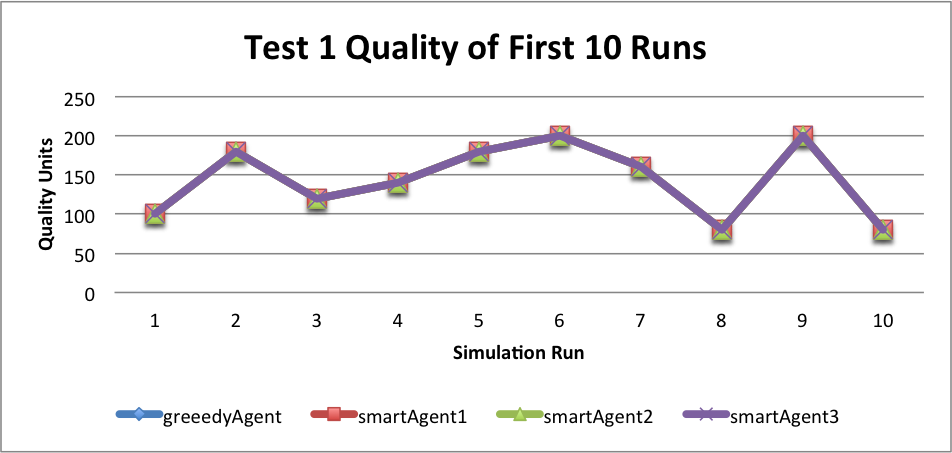
\includegraphics[width=10cm]{images/Test1Q.png}
\caption{All four agents were able to achieve identical quality throughout the first 10 runs of the simulation}
\label{fig:Test1Q}
\end{figure}

\begin{figure}[H]
\centering
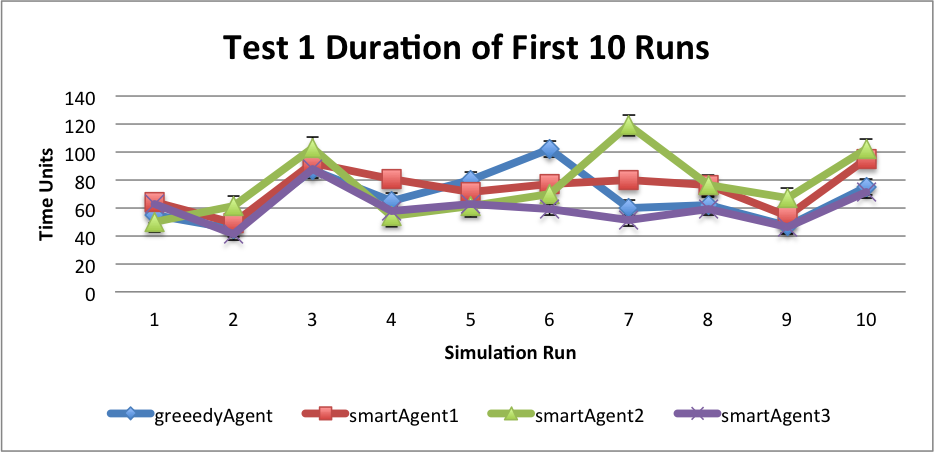
\includegraphics[width=10cm]{images/Test1D.png}
\caption{The results indicate that smartAgent3 was able to navigate the simulation the fastest while still achieving the maximum possible quality. }
\label{fig:Test1D}
\end{figure}

\begin{figure}[H]
\centering
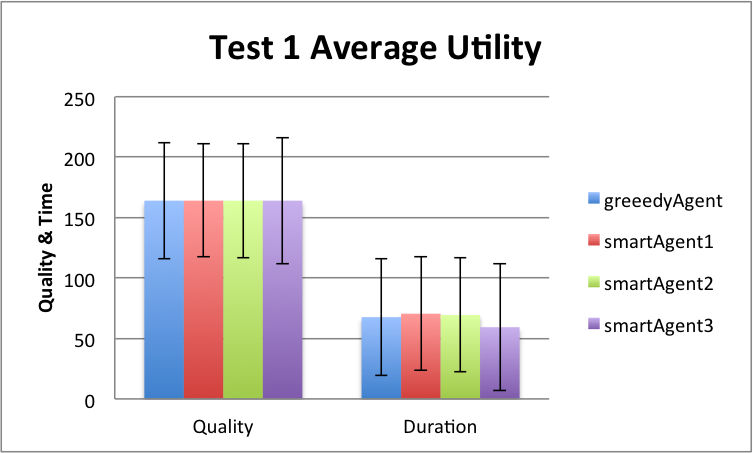
\includegraphics[width=10cm]{images/Test1A.png}
\caption{This figure shows the average quality and duration for each agent across all 25 runs of Test 1.}
\label{fig:Test1A}
\end{figure}


}


\item{\textbf{Test 2}

As seen in Figure \ref{fig:Tree2}, Test2.ctaems consists of four tasks and 13 methods in which 12 of the tasks were divided between three agents. This setup ensured that the forth agent who was responsible for only one method had the minimal load. The experiment tested the agent's ability to load balance in order to decrease the time required to complete the simulation. Figure \ref{fig:Test2D} shows the greedy agent is unable to load balance and therefore takes significantly longer to complete the simulation.

\begin{figure}[H]
\centering
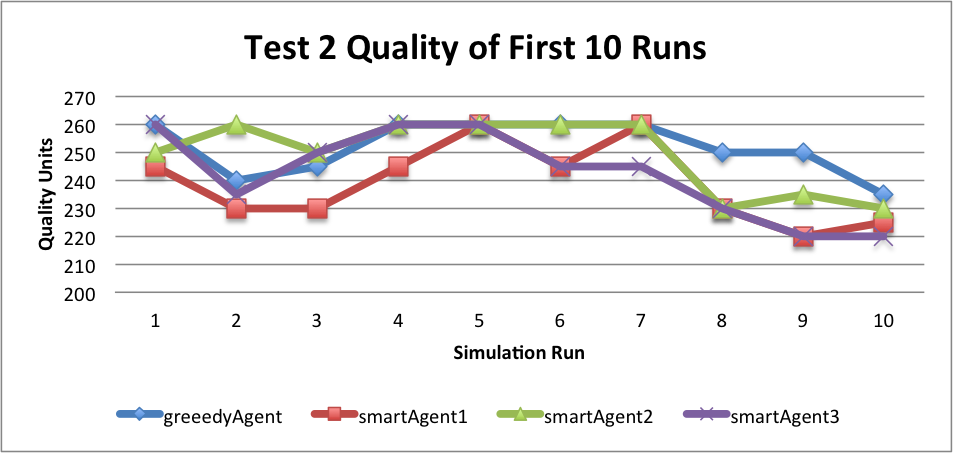
\includegraphics[width=10cm]{images/Test2Q.png}
\caption{All four agents were able to achieve similar quality throughout the first 10 runs of the simulator.}
\label{fig:Test2Q}
\end{figure}

\begin{figure}[H]
\centering
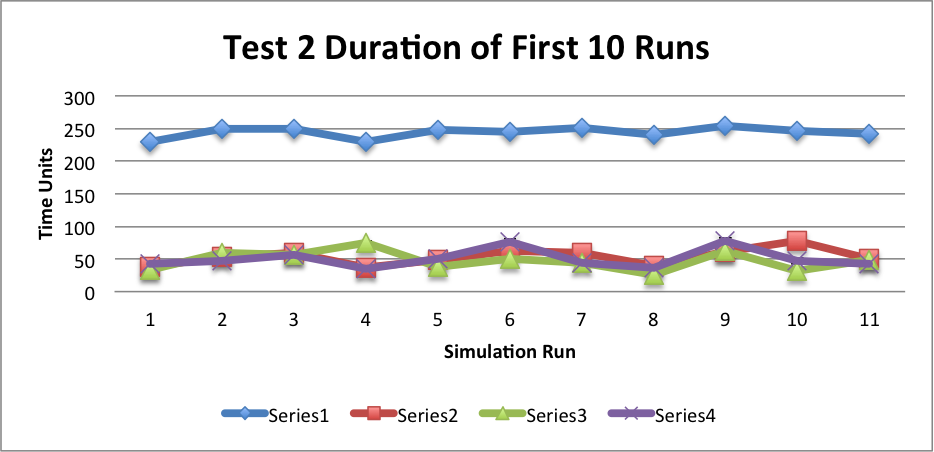
\includegraphics[width=10cm]{images/Test2D.png}
\caption{The results indicate that greedy agent was unable to load balance resulting in additional time required to complete the simulation }
\label{fig:Test2D}
\end{figure}

\begin{figure}[H]
\centering
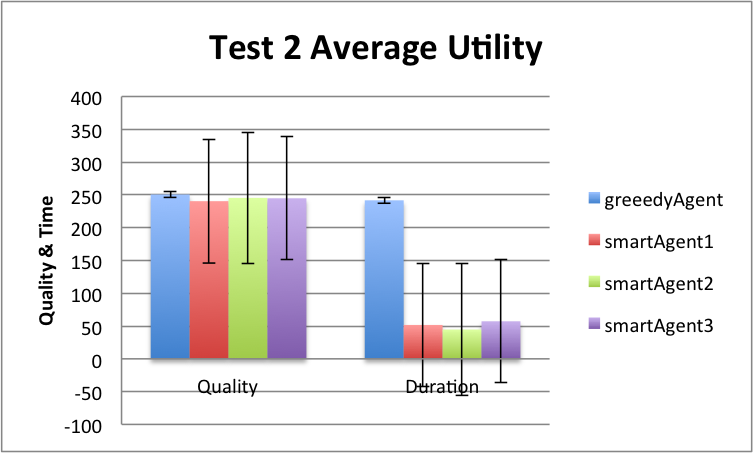
\includegraphics[width=10cm]{images/Test2A.png}
\caption{This figure shows the average quality and duration for each agent across all 25 runs of Test 2.}
\label{fig:Test2A}
\end{figure}

}


\item{\textbf{Test 3}

As seen in Figure \ref{fig:Tree3}, Test3.ctaems consists of four tasks and 16 methods designed in a way that a greedy agent would not be optimal. The results confirm this design. Figure \ref{fig:Test3A} shows that the greedy agent achieved the least quality where smartAgent2 and smartAgent3 were able to achieve a greater quality. The duration results shown in Figure \ref{fig:Test3D} are also interesting and serve to confirm that the later generations of agents were not only able to achieve better quality, but do so in less time. This is because the smart agents are able to cooperate to determine a more efficient path through the simulation. 

\begin{figure}[H]
\centering
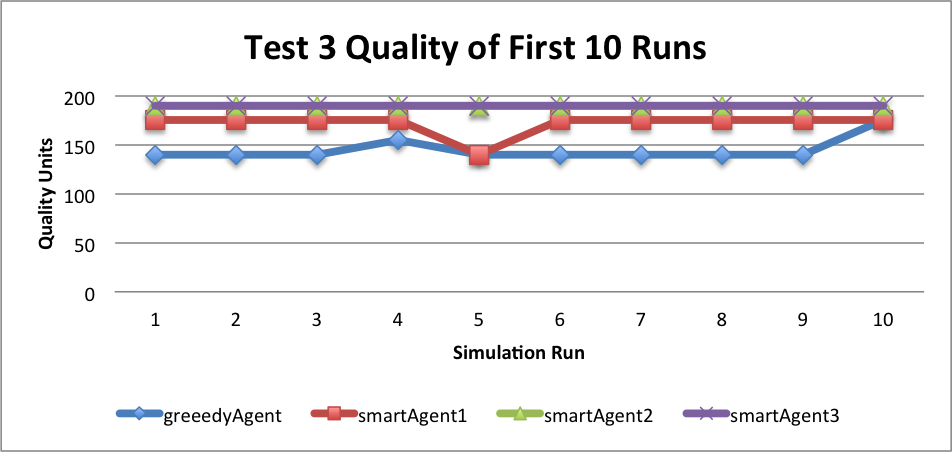
\includegraphics[width=10cm]{images/Test3Q.png}
\caption{This figure shows the ability of the more advanced agents to act in a cooperative manner to achieve additional utility that was abandoned by the greedy agent.}
\label{fig:Test3Q}
\end{figure}

\begin{figure}[H]
\centering
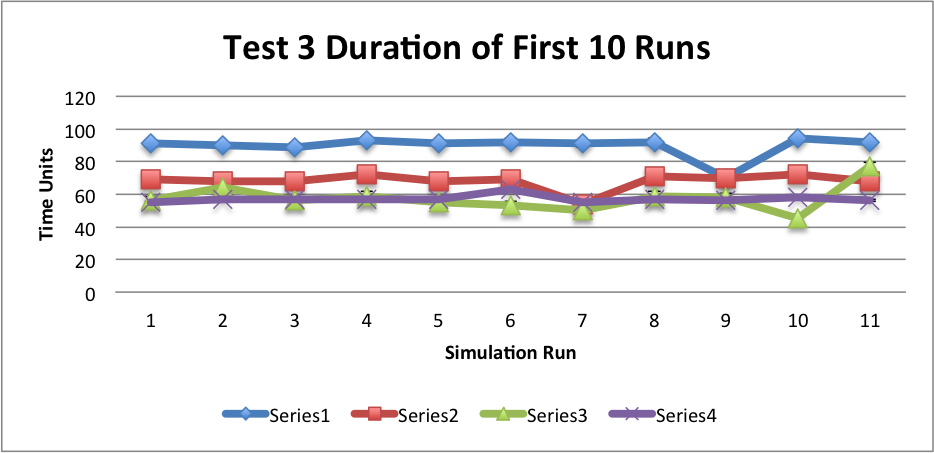
\includegraphics[width=10cm]{images/Test3D.png}
\caption{The results indicate that the more advanced agents were able to navigate the simulation faster and achieve additional utility. }
\label{fig:Test3D}
\end{figure}

\begin{figure}[H]
\centering
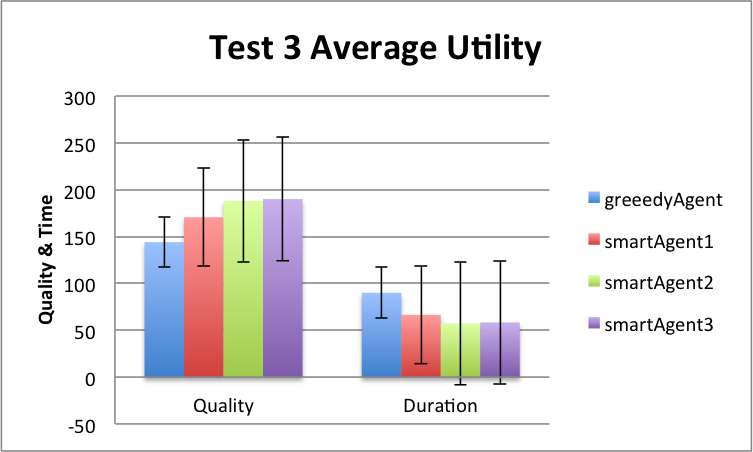
\includegraphics[width=10cm]{images/Test3A.png}
\caption{This figure shows the average quality and duration for each agent across all 25 runs of Test 3.}
\label{fig:Test3A}
\end{figure}
}
\item{\textbf{Test 4}
As seen in Figure \ref{fig:Tree4}, Test3.ctaems consists of four tasks and 16 methods as well as several disables and facilitates relationships. In this experiment, the negative effect of poor choices is increased through use of the disables relationship type. Although I expected only smartAgent3 to be able to achieve the maximum utility, smart agent one did surprisingly well. This is because it used the load balancing heuristic the complete methods 5, 10, and 15 before the disables relationships could take effect. This unexpected result also allowed smartAgent1 to achieve the fastest time of any agent as seen in Figure \ref{fig:Test4D}. Althogh smartAgent3 was also able to achieve considerable utility by pre-planning it's path, it was unable to complete the simulation as quickly. 

\begin{figure}[H]
\centering
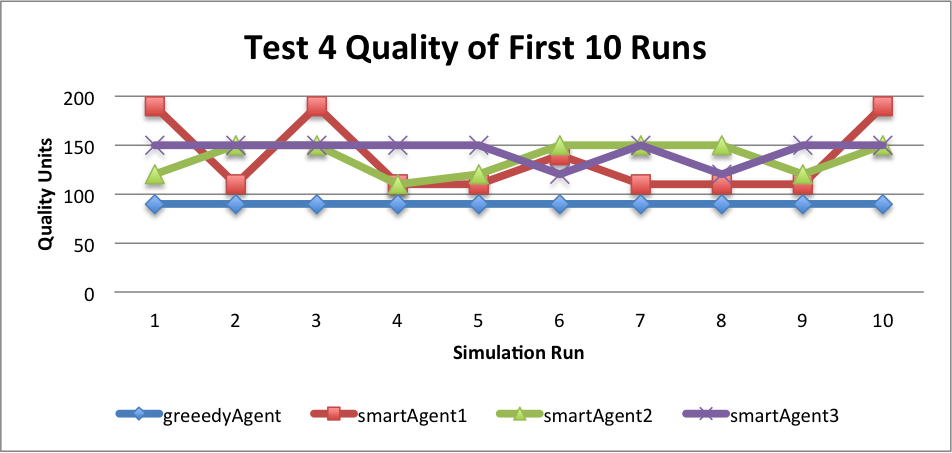
\includegraphics[width=10cm]{images/Test4Q.png}
\caption{Unexpectedly, smartAgent1 was able to use load balancing to achieve a considerable quality result.}
\label{fig:Test4Q}
\end{figure}

\begin{figure}[H]
\centering
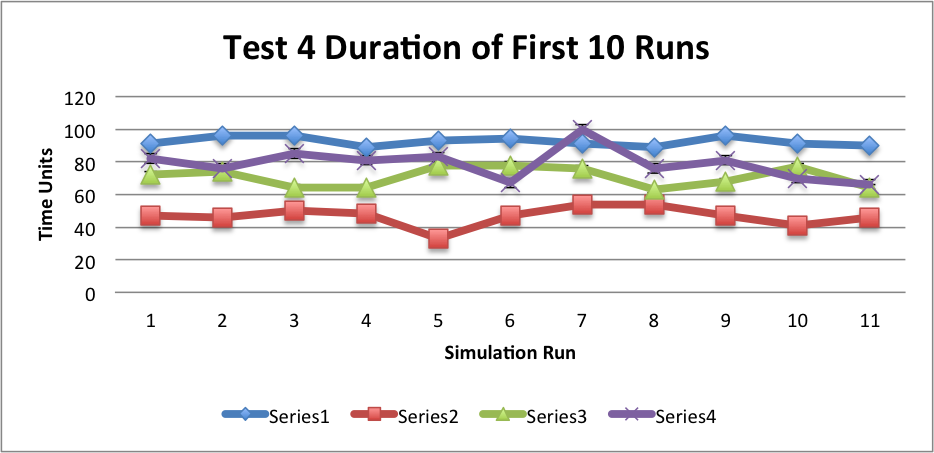
\includegraphics[width=10cm]{images/Test4D.png}
\caption{SmartAgent1's use of load balancing allowed it to navigate the simulation quicker then the planning agents. }
\label{fig:Test4D}
\end{figure}

\begin{figure}[H]
\centering
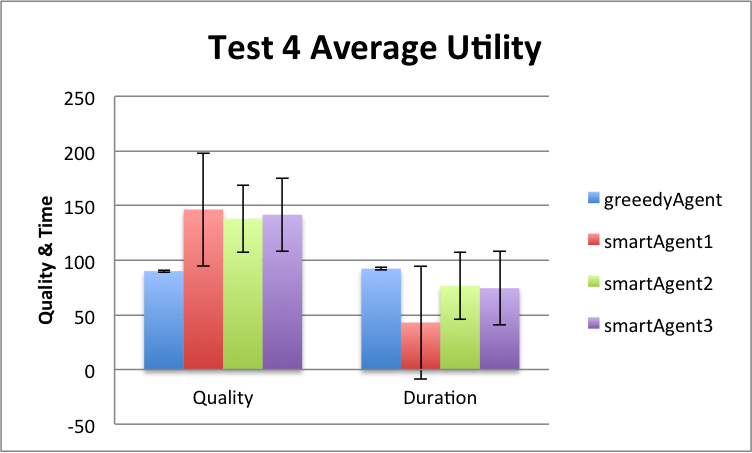
\includegraphics[width=10cm]{images/Test4A.png}
\caption{This figure shows the average quality and duration for each agent across all 25 runs of Test 4.}
\label{fig:Test4A}
\end{figure}


}
\end{itemize}

\end{itemize}


\end{document}
